\scanpage{75}
\[
\sum_1^n\log(1+r\rho_i(u+v))\leq\sum_1\log(1+r\rho_i(u))+\sum_1\log(1+r\rho_i(v))
\]

\[
S_{\deleted{\unsure{m}}\varphi}^{n}(u+v)\leq S_\varphi^n(u)+S_\varphi^n(v)\qquad S_\varphi^n(w)=\sum_1^n f_\varphi(\rho_i(w))
\]

\[
f_\varphi(\rho)=\int_0^{+\infty}\frac{\varphi(r)}{\frac1\rho+r}\,dr=\int_0^{+\infty}\varphi\left(\frac s\rho\right)\frac{ds}{1+s}
\]

$\varphi$ fonction décroissante

(motivation : \inserted{Si $A(0)=B(0)=0$ ($=0$ est un \unsure{symbole|exemple}), alors} $A(r)\leq B(r)$ pour $0\leq r\leq+\infty$ équivaut à $\int\psi(r)A(r)\,dr\leq\int\psi(r)B(r)\,dr$ pour toute $\psi\geq0$ à support cp\textsuperscript{t} dans $[a,b]$, Or, en posant $\psi(r)=-\varphi'(r)$, $\varphi$ fonction \unsure{décroissante} \inserted{\uline{continûment} \uline{différentiable}}, nulle en $b$ : \deleted{(\unsure{continûment}} \unsure{\deleted{\inserted{nulle}}|\inserted{nulle}} \deleted{\unsure{continue au} \illegible{1}} (ce qui est $+\infty$) et supposant \deleted{\unsure{de}}

que $A$ est dérivable $-\int\varphi'(r)A(r)\,dr=[-\varphi(r)A(r)]_0^{+\infty}+\int\varphi(r)A'(r)\,dr$ et le premier terme est nul, d'où $\int\varphi(r)A'(r)\,dr$. Si donc $A$ et $B$ sont dérivables, alors on obtient donc

\[
\int\varphi(r)A'(r)\,dr\leq\int\varphi(r)B'(r)\,dr
\]

pour toute fonction $\varphi$ continûment différentiable, décroissante \inserted{sur $[0,+\infty[$} et nulle au voisinage de $+\infty$. Si en plus $A'(r)$, $B'(r)\geq0$, alors ça sera vrai pour \deleted{toute} fonction décroissante \unsure{telle} ou nulle, pouvant être infinie. (Si on prend

$\varphi=$

\figure{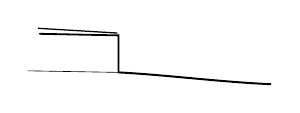
\begin{tikzpicture}[x=1mm,y=1mm,line cap=round]\draw[line width=.16mm] (0,5.6)--(10,5.0);\draw[line width=.23mm] (.2,4.9)--(10.2,4.7)--(10.2,0);\draw[line width=.08mm] (-1.3,.2)--(10.2,0);\draw[line width=.25mm] (10.2,0)..controls(16,-.3)and(23,-1.2)..(29.5,-1.5);\end{tikzpicture}}

, on retrouve $A(r)\leq B(r)$). Dans le cas actuel,

\[
A\deleted{\unsure{^{\,\prime}|{}^{\sim}}}(r)=\sum_1^n\log(1+r\rho_i(u))\qquad \text{donc }\ A'(r)=\sum\frac{r}{1+r\rho_i(u)}
\]

d'où notre assertion. -- Le cas le plus important est celui où on prend $\varphi(r)=r^{-p}$ $0<p<1$. On trouve alors

\margin{76}
